\documentclass[conference]{IEEEtran}

\usepackage[pdftex]{graphicx}
\graphicspath{{../pdf/}{../jpeg/}}
\DeclareGraphicsExtensions{.pdf,.jpeg,.png}

\renewcommand{\arraystretch}{1.3}
\usepackage{etoolbox}
\apptocmd{\thebibliography}{\setlength{\itemsep}{3pt}}{}{}

\usepackage{url}

\hyphenation{op-tical net-works semi-conduc-tor}


\begin{document}

\title{Reconfigurable Self-timed Dataflow Accelerator \\\& Fast Network Analysis in Silicon}

\author{$\mu$Systems Group, School of Electrical and Electronic Engineering, Newcastle University, UK}

\maketitle

\iffalse
\begin{abstract}
Many real-life applications require dynamically reconfigurable pipelines to handle incoming data items differently depending on their values or current operating mode. Reconfigurable asynchronous pipelines have neither a formal behavioural model, nor mature automation support. An asynchronous accelerator for ordinal pattern encoding, with reconfigurable pipeline depth, is shown. This has been designed, simulated and verified using the dataflow structure model of the EDA tool Workcraft; then fabricated using the TSMC 90nm technology.

Applications that rely on underlying graph models foster the importance of having a fast and flexible approach to graph analysis. In order to support medicine discovery, biological systems are modelled by graphs, and drugs can disconnect some of the internal connections. Graphs are automatically converted into VHDL designs, which are synthesised into an FPGA for the analysis. Thousand times faster than in software. We will demo the projects using one stand.
\end{abstract}
\fi

\IEEEpeerreviewmaketitle

%\noindent
%We intend to demo the two projects discussed in this document using one single stand.

\section*{Reconfigurable self-timed dataflow accelerator}
Many real-life applications require dynamically
reconfigurable pipelines to handle incoming data items differently depending on their values
or the current operating mode. Reconfigurable synchronous
pipelines are known since 1980s and are well
supported by formal models and EDA tools. Reconfigurable asynchronous
pipelines on the other hand, have neither a formal behavioural model, nor
mature automation support, making them unattractive to industry.

We will demo an asynchronous accelerator for ordinal pattern encoding~\cite{OPE} with
reconfigurable pipeline depth. The hardware system has been designed, verified and synthesised
using the \emph{dataflow structure} model~\cite{DFS} in \textsc{Workcraft}~\cite{workcraft_web}. This approach has been
then validated with the fabrication of an ASIC (TSMC 90nm technology) via
Europractice.

\begin{figure}[ht!]
%\vspace{-3mm}
\begin{center}
	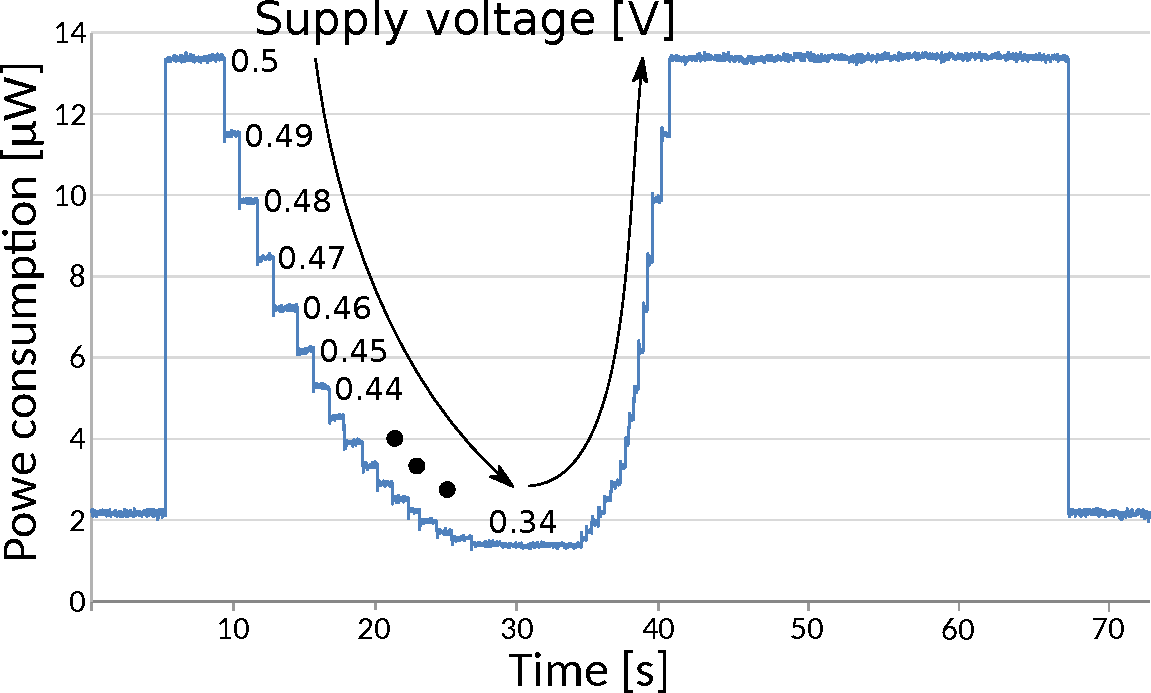
\includegraphics[width=\linewidth]{FIG/voltage-var.pdf}
	\caption{Voltage variation resilience.}
	\label{fig:voltage-var}
\end{center}
%\vspace{-5mm}
\end{figure}

\noindent
The chip has been equipped with a testing infrastructure to collect statistics for future research. The most interesting results are: 
\begin{itemize}
\item High resilience of self-timed circuit to voltage variation~(0.3 - 1.6V), see Figure~\ref{fig:voltage-var} for sub-threshold measurements. This enables another degree of optimisation for energy/time interplay.
\item Energy consumption and computation time can be dynamically regulated by the depth of the pipeline.
\item The cost of reconfigurability, in terms of area, computation time and energy consumption is negligible compared to the non-reconfigurable reference design.
\item The \emph{dataflow structure} plugin of \textsc{Workcraft} supports the design, simulation, verification of asynchronous reconfigurable pipelines.
\end{itemize}

\section*{Fast network analysis in silicon}
The importance of having a fast and flexible approach to the analysis of networks is given by
the high number of applications that rely on underlying graph-based models. In our case study,
biological systems are modelled by graphs, and drugs can disconnect some of the connections
within them. Parameters such as the average shortest path gives the resilience to a particular
drug, and help analyse the effectiveness of a medicine. In software, graph analysis is
computationally expensive: the internal paths should be explored one at a time. 
The maximum performance can be obtained by mapping the whole network into a piece of silicon
and exploiting the hardware parallelism completely. In our demo, a network (defined as an XML
file) can be automatically converted into a HDL design where the nodes are modelled with
registers, and connections with wires. The network is then placed into a pre-designed system
for the analysis, Figure~\ref{fig:fantasi}. The whole design is synthesised into Altera
FPGA-based board. FPGAs fit this application well, providing the right tradeoff between speed
and flexibility. The developed accelerator is to be integrated into the drug discovery flow of
our industrial partner.

\begin{figure}[ht!]
%\vspace{-1mm}
\begin{center}
	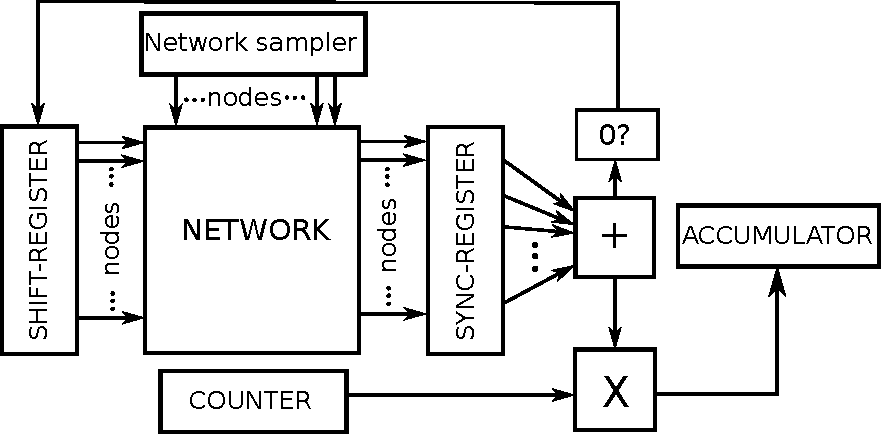
\includegraphics[width=\linewidth]{FIG/fantasi+.pdf}
	\caption{Hardware system for fast network analysis.}
	\label{fig:fantasi}
\end{center}
%\vspace{-1mm}
\end{figure}
\noindent
The demo will include:
\begin{itemize}
\item The flow from the network conversion to the analysis.
\item The comparison between the C++ software implementation of the analysis algorithm and the
hardware counterpart (thousands times faster).
\item Statistics gathered from different networks.
\end{itemize}

\begin{thebibliography}{3}
\scriptsize
\bibitem{OPE}
	C. Guo et al.
	\emph{``Pipelined reconfigurable accelerator for ordinal pattern encoding''}.
	ASAP, 2014.

\bibitem{DFS}
	D. Sokolov et al. \emph{``Analysis of static data flow structures''}.
	Fundamenta Inf., 2008.

\bibitem{workcraft_web}
	\textsc{Workcraft} homepage. \url{http://www.workcraft.org/}.	

\end{thebibliography}

\end{document}
